\mode*

\begin{frame}
\frametitle{Example: Partially Linear Regression}
%\begin{block}{Partially Linear Regression model (PLR)}
%\textbf{Partially linear regression} models take the form

\begin{itemize}
\item Partially linear regression (PLR) model
\begin{align*}
&Y = D \theta_0 + g_0(X) + \zeta, & &\mathbb{E}[\zeta | D,X] = 0, 
\end{align*}
with potentially non-linear function $g_0()$ and
%\vspace*{-20pt}
%\end{block}
\begin{itemize}
\item Outcome variable $Y$
\item Policy or treatment variable of interest $D$
\item High-dimensional vector of confounding covariates $X = (X_1, \ldots, X_p)$
%\item Stochastic errors $\zeta$ and $V$
\end{itemize}
\end{itemize}
%\vspace{10pt}
%\begin{center}
%\pdftooltip{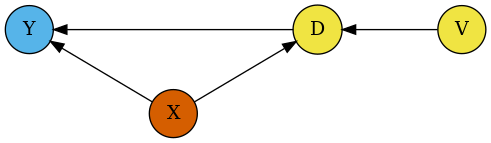
\includegraphics[width=0.6\textwidth]{pictures_and_logos/dag_plr2.png}}{A graph illustrating the  partially linear regression setting. There are four nodes in total: One for the dependent variable Y, one for the treatment variable D, one for the vector of confounding variables X and one for the stochastic error V. There are four directed edges in the figure, each illustrating a causal channel: From V into D, from D into Y, from X into Y and from X into D.}
%\end{center}
\end{frame}

\begin{frame}
\frametitle{Problems in Naive Approaches}
\begin{itemize}
\item Failure of naive approaches: \textbf{Regularization bias}, e.g.,
\begin{itemize}
\item Naive variable selection, for example based on the lasso
\item Naive plug-in predictions, for example from random forests
\end{itemize}
\end{itemize}
\vspace{10pt}
\begin{center}
\pdftooltip{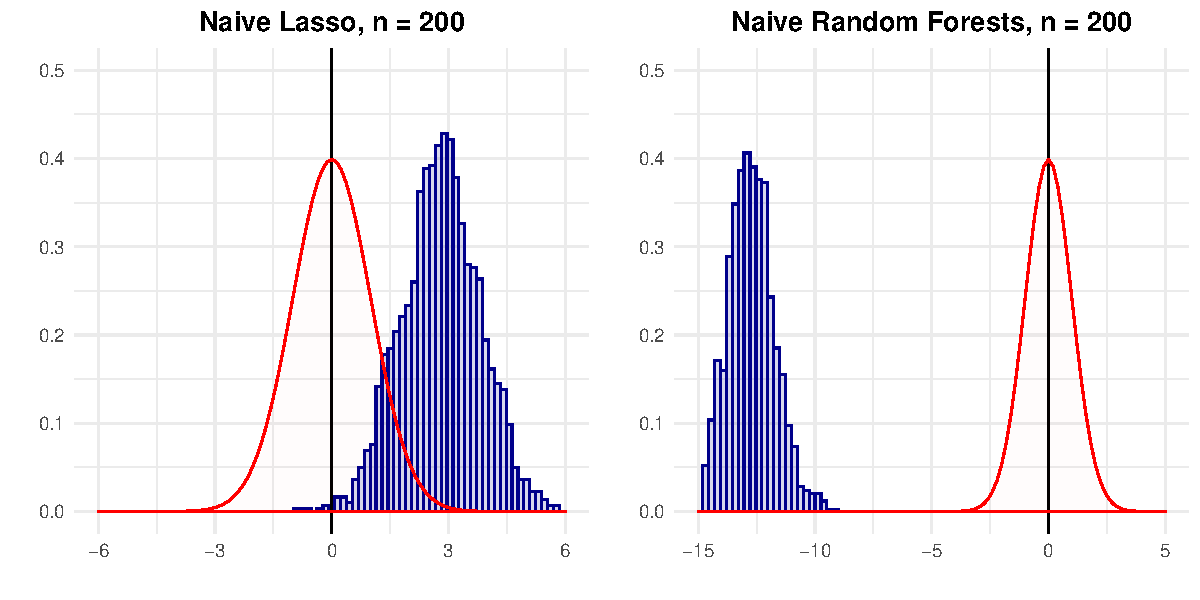
\includegraphics[width=0.8\textwidth]{pictures_and_logos/comp_naive_ml_resc_n200_p200.pdf}}{The figure shows two histograms of the empirical distribution (blue bars) of two naive machine learning estimators for THETANULL in a simulation example. The estimators are studentized, i.e., the true value of THETANULL is subtracted from the value of the estimator and this difference is then divided by the empirical standard deviation of the simulated estimators. The histogram on the left hand side corresponds to estimation of THETANULL that is based on naive variable selection by the lasso, i.e., only those variables in the PLR are included that have been selected in a lasso regression. The histrogram on the right hand side corresponds to a random forest learner which is trained to generate predictions for the outcome Y using covariates X. These predictions are then simply plugged in into the PLR regression equation. In both cases the empirical distribution substantially differs from a normal distribution. In both figures, the density of a standard normal random variable is illustrated by a red curve, which is symmetric around zero. As opposed to the shape of this density, both histograms are not centered at zero, which illustrates a severy bias. In case of the lasso, the estimator is upward biased and in case of the random forest estimator, the estimator is downward biased. Moreover the empirical distributions do not appear symmetric.}
\end{center}
\end{frame}


%\begin{frame}
%\frametitle{Data Generating Process}
%\begin{itemize}
%\item \textbf{Partially linear regression} model
%\vspace*{-10pt}
%\begin{align*}
%&y_i = d_i \theta_0 + g_0(x_i) + \zeta_i, \\
%&d_i = m_0(x_i) + v_i,
%\end{align*}
%with $\zeta_i, v_i \sim \mathcal{N}(0,1)$ and $x_i \sim \mathcal{N}_{p}(0, \Sigma)$.
%\item Variance-covariance matrix $\Sigma$ with entries $\Sigma_{kj} = 0.7^{|j-k|}$
%\item True parameter $\theta_0 = 0.5$
%\item \textbf{Non-linear nuisance functions}
%\vspace*{-5pt}
%\begin{align*}
%&g_0(x_i) = \frac{\exp(x_{i1})}{1+\exp(x_{i1})} + \frac{1}{4} x_{i3} \\
%&m_0(x_i) = x_{i1} + \frac{1}{4} \frac{\exp(x_{i3})}{1+\exp(x_{i3})}
%\end{align*}
%\item $n=500$ observations and $p=20$ explanatory variables
%\end{itemize}
%\end{frame}
%
%
%
%\begin{frame}
%\frametitle{Regularization Bias in Simple ML-Approaches}
%\textbf{Naive} prediction-focused \textbf{ML approach} (Don't do it!):
%\begin{itemize}
%\item Fit a random forest (or another ML method) to predict $Y$ based on the features $X$, i.e., estimate $g_0(X)$
%\item Given $\hat{g}_0(X)$, the final estimate of $\theta_0$ is obtained as ($n=N/2$)
%\end{itemize}
%\vspace*{-7pt}
%\begin{align*}
%\hat{\theta}_0 = \left(\frac{1}{n} \sum_{i\in I} D_i^2\right)^{-1} \frac{1}{n} \sum_{i\in I} D_i (Y_i - \hat{g}_0(X_i))
%\end{align*}
%\vspace*{-7pt}
%\begin{itemize}
%\item Driving factor for the \textbf{regularization bias}: \textbf{Bias in learning $g_0$}
%\end{itemize}
%\begin{columns}
%\hspace*{12pt}
%\begin{column}{0.5\textwidth}
%\includegraphics[height=0.75\textwidth]{../../../paper_py_pkg/sim/presentation/predictions.png}
%\end{column}
%\begin{column}{0.5\textwidth}
%\includegraphics[height=0.75\textwidth]{../../../paper_py_pkg/sim/presentation/nonorth.png}
%\end{column}
%\end{columns}
%\end{frame}

%
%\begin{frame}
%\frametitle{Overcoming Regularization Bias by \\Orthogonalization}
%\begin{itemize}
%\item Directly \textbf{partialling out} the effect of $X$ from $D$ to obtain the \textbf{orthogonalized} regressor $V = D - m_0(X)$
%\item Use the final estimate
%\begin{align*}
%\hat{\theta}_0 = \left(\frac{1}{n} \sum_{i\in I} \hat{V}_i \hat{V}_i\right)^{-1} \frac{1}{n} \sum_{i\in I} \hat{V}_i (Y_i - \hat{g}_0(X_i))
%\end{align*}
%\end{itemize}
%\begin{center}
%\includegraphics[width = 0.45\textwidth]{../../../paper_py_pkg/sim/presentation/orth.png}
%\end{center}
%\end{frame}
%
%\begin{frame}
%\frametitle{Sample Splitting to Remove Bias Induced \\by Overfitting}
%\begin{itemize}
%\item If the nuisance models $\hat{g}_0$ and $\hat{m}_0$ are estimated on the whole dataset, which is also used for obtaining the final estimate $\hat{\theta}_0$, another \textbf{bias induced by overfitting} can be observed
%\end{itemize}
%\begin{center}
%\includegraphics[width = 0.45\textwidth]{../../../paper_py_pkg/sim/presentation/nosplit.png}
%\end{center}
%\end{frame}
%
%
%\begin{frame}
%\frametitle{Sample Splitting to Remove Bias Induced \\by Overfitting}
%\begin{itemize}
%\item Use \textbf{sample splitting} to overcome the \textbf{bias induced by overfitting}, i.e.,
%\begin{itemize}
%\item Estimate the nuisance models $\hat{g}_0$ and $\hat{m}_0$ on one part of the data (training data)
%\item Estimate $\hat{\theta}_0$ on the other part of the data (test data)
%\end{itemize}
%\end{itemize}
%\begin{center}
%\includegraphics[width = 0.45\textwidth]{../../../paper_py_pkg/sim/presentation/dml.png}
%\end{center}
%\end{frame}
%
%\begin{frame}
%\frametitle{Sample Splitting to Remove Bias Induced \\by Overfitting}
%\begin{itemize}
%\item \textbf{Cross-fitting} performs well empirically (efficiency gain by switching roles)
%\end{itemize}
%\begin{columns}
%\hspace*{12pt}
%\begin{column}{0.5\textwidth}
%\includegraphics[height=0.8\textwidth]{../../../paper_py_pkg/sim/presentation/orth_theta.png}
%\end{column}
%\begin{column}{0.5\textwidth}
%\includegraphics[height=0.8\textwidth]{../../../paper_py_pkg/sim/presentation/dml_theta.png}
%\end{column}
%\end{columns}
%\end{frame}
%
%
%\begin{frame}
%\frametitle{Comparison of All Approaches}
%
%\begin{center}
%\includegraphics[width=0.95\textwidth]{../../../paper_py_pkg/sim/presentation/all.png}
%\end{center}
%\end{frame}
